\section{Filtering the corpus}
\label{sec:ppot:classifier}

As discussed in Section \ref{subsec:ppot:download-policies}, we expect that some of the downloaded pages are not privacy policies. In order to filter out web pages that are not privacy policies, we trained a classifier on manually labeled data from the candidate policies. In this section, we refer to the text of the crawled web pages extracted with \emph{html2text} as \textit{documents}.

\textbf{Labeling definition.}
\label{subsec:ppot:pp-definition}
In order to label documents as privacy policies (or not), we needed to adopt a definition of what constitutes a privacy policy. We did not select a definition based on legal requirements, since both privacy policy text and applicable law can be ambiguous; we considered it outside the scope of the project to develop a classifier that accurately determines whether a document satisfies relevant legal requirements. Moreover, different jurisdictions have different legal requirements, which would necessitate further judgment about the applicable law for a given website.

Instead, we aimed to label whether a document is an \textit{apparent} privacy policy, without determining whether the document meets any particular legal requirements. Specifically, we labeled a document as a privacy policy if it met all of the following criteria:
\begin{itemize}
    \item The document relates to privacy. This criterion eliminates documents that are irrelevant, notwithstanding the link text.
    \item The document is legal in nature (e.g., uses legal terminology or appears to have legal significance). This eliminates documents that informally discuss privacy, such as blog posts.
\end{itemize}
In the course of applying our criteria, we encountered several recurring borderline types of documents. We labeled the following categories of documents as not privacy policies, because the contents were dissimilar or could otherwise be problematic for automated textual analysis.
\begin{itemize}
\item Incomplete privacy policies.

\item Cookie policies, which only describe the privacy practices of the website with respect to cookies.

\item Security policies, which only describe the security practices of the website.

\item Mixed documents containing paragraphs that are unrelated to privacy, such as a privacy policy intertwined with terms of service.

\item Privacy centers or landing pages, which further link to a privacy policy.

\item Privacy policy summaries, which further link to a long-form privacy policy.

\end{itemize}

\textbf{Labeling the sample.} We started by manually labeling a sample of candidate privacy policies (i.e., documents returned by the crawler) using our criteria. First, we randomly sampled and labeled 1,139 documents. In the sample, the majority of the documents 
matched the ``privacy + policy'' link text pattern (as described in Section \ref{subsec:ppot:download-policies}). We additionally sampled 50 random documents for each of the six remaining link text patterns so as to reduce overrepresentation of the 
dominant
link text pattern.

To confirm that the labeling was consistent with our criteria, two researchers independently labeled a sample of 100 randomly collected documents using the criteria above. The inter-annotator agreement was $\kappa=0.93$.

Our final labeled dataset contains 1,173 positives (i.e., documents that are privacy policies) and 266 negatives (i.e., documents that are not privacy policies), respectively $\sim$81.5\% and $\sim$18.5\%.

\textbf{Converting documents to features.} We cleaned the documents by removing Markdown tags and retaining inner text. We then removed symbols and the set of English stop words in \emph{scikit-learn}~\cite{scikit-learn}. Next, we created word n-gram tokens spanning from unigrams to 4-grams and generated features based on the frequency of occurrence of each token. We excluded tokens that appeared in fewer than 1\% of the documents.

We also extracted features from document titles, parsing them from the HTML \texttt{<title>} tag. For PDF files, we obtained titles by using the \textit{pdftitle} library~\cite{pdftitle-pypi}.
We removed symbols and stop words from the titles and we generated features based on the number of occurrences of each unigram in the title. We excluded tokens that appeared in fewer than 1\% of the documents.

We additionally extracted features from the link text and document URL. We found that these features did not contribute to classification performance, so we excluded them from our model.

\begin{figure}[]
\centering
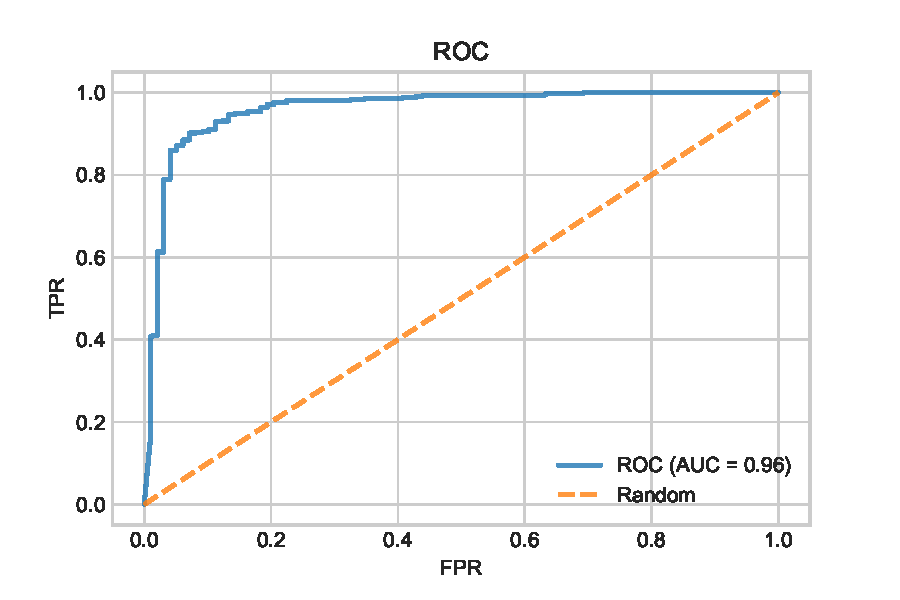
\includegraphics[width=0.8\columnwidth]{chapters/privacypolicies/figures/roc.pdf}
\caption[Predictive performance of the privacy policy random forest classifier]{Predictive performance of the privacy policy random forest classifier, applied to held-out documents.}
%\Description[ROC curve]{An ROC curve, with an AUC of 0.96}
\label{fig:roc-auc}
\end{figure}

\textbf{Model training and validation.}
We trained and tested two model types, random forest and logistic regression, using 10-fold cross validation across varying hyperparameters. We evaluated the models based on maximizing average area under the receiver operating characteristic curve (\textit{AUC}), since that metric accounts for the class imbalance. The best performing random forest model had a higher mean AUC than the best performing logistic regression model (97\% vs. 95\%), so we selected the random forest model.

We then considered the tradeoff between precision and recall for the random forest model. We manually selected a classification threshold that prioritized precision over recall, since we anticipate uses of our corpus (e.g., many forms of automated analysis) that may be more sensitive to erroneously including non-privacy policy documents than erroneously omitting privacy policies.

Finally, we evaluated our model on a held-out set of 749 randomly sampled and manually labeled documents, consisting of 651 positives and 98 negatives. The performance of the final model on the held-out set is shown in Figure \ref{fig:roc-auc}. The chosen classification threshold resulted in 97.9\% precision and 94.2\% recall.

\textbf{Document Classification.}
Approximately 17\% (220,932) of the documents in the dataset were classified as negatives, with the final dataset totaling 1,071,488 policies. We discuss the release of this data in Section \ref{sec:ppot:conclusion}.

